% --------------------------------------------------------------
% This is all preamble stuff that you don't have to worry about.
% Head down to where it says "Start here"
% --------------------------------------------------------------
 
\documentclass[12pt]{article}

\usepackage[margin=1in]{geometry} 
\usepackage{amsmath,amsthm,amssymb,listings,xcolor,graphicx, subfig, subcaption, enumerate,framed}
 
\newenvironment{solution}{\begin{proof}[Solution]}{\end{proof}}

\definecolor{codegreen}{rgb}{0,0.6,0}
\definecolor{codegray}{rgb}{0.5,0.5,0.5}
\definecolor{codepurple}{rgb}{0.58,0,0.82}
\definecolor{backcolour}{rgb}{0.97,0.97,0.97}
\lstdefinestyle{pystyle}{
    backgroundcolor=\color{backcolour},   
    commentstyle=\color{codegreen},
    keywordstyle=\color{magenta},
    numberstyle=\tiny\color{codegray},
    stringstyle=\color{codepurple},
    basicstyle=\ttfamily\small,
    breakatwhitespace=false,         
    breaklines=true,                 
    captionpos=b,                    
    keepspaces=true,                 
    numbers=left,                    
    numbersep=5pt,                  
    showspaces=false,                
    showstringspaces=false,
    showtabs=false,                  
    tabsize=2
}
\lstset{style=pystyle}

\graphicspath{{./figures}}
 
\begin{document}
 
\title{Homework 5: The DCT and JPEG Compression}
\author{Matthew Luyten\\
ECE6250}

\maketitle

\begin{enumerate}
\item[Problem 5.1] Summary and Context of the Discrete Cosine Transform and JPEG Compression

This week, we finally got to apply the weeks of theory and linear algebra and use it to understand
a 30-year old image compression technique. While studying orthobases and orthogonal projections
felt like an excessive digression into theory, I see now that we needed those building blocks to
understand cosine and wavelet transforms. JPEG is still a very common image compression technique,
and it's algorithm is pretty simple to understand with the background understanding we've built up.

We also compared the DCT to the FFT and gained insight into the ways we can use the FFT to quickly
perform the DCT. Recognizing these similarities and applying them in a practical scenario is an
important skill for an engineer. The FFT algorithm is fast and ubiquitous, so it's a handy tool
to keep around.

Seeing JPEG's my whole life, I'll admit that I was very excited that we got to implement our own
JPEG-ish transform. To quote rapper and producer JPEGMAFIA's iconic producer tag:

"I named this one JPEG, because I like JPEG's, uh, for the resolution, the color, the size of them.
Everything about JPEG's I like" (HERMANOS, JPEGMAFIA)

\newpage

\item[Problem 5.2] JPEG Concepts

\begin{enumerate}

\item[a.] Block DCT2 Function:
\begin{lstlisting}[language=matlab]
function XB = block_dct2(IM, N)
    dim = size(IM);
    XB = zeros(dim(1), dim(2));
    for i = 1:dim(1) / N
        for j = 1:dim(2) / N
            XB((i-1)*N+1:i*N, (j-1)*N+1:j*N) = dct2(IM((i-1)*N+1:i*N, (j-1)*8+1:j*N));
        end
    end
end
\end{lstlisting}

Block IDCT2 Function:
\begin{lstlisting}[language=matlab]
function IM = block_idct2(XB, N)
    dim = size(XB);
    IM = zeros(dim(1), dim(2));
    for i = 1:dim(1) / N
        for j = 1:dim(2) / N
            IM((i-1)*N+1:i*N, (j-1)*N+1:j*N) = idct2(XB((i-1)*N+1:i*N, (j-1)*N+1:j*N));
        end
    end
end
\end{lstlisting}

\item[b.] DCT2 Approximation Function:
\begin{lstlisting}[language=matlab]
function IM_C = block_dct2_approx(IM, M)
    N = 8;
    coeffs = block_dct2(IM, N);
    dim = size(coeffs);
    [z, pairs, map] = jpgzzind(N, N);
    mask = map <= M;
    for i = 1:dim(1) / N
        for j = 1:dim(2) / N
            coeffs((i-1)*N+1:i*N, (j-1)*N+1:j*N) = coeffs((i-1)*N+1:i*N, (j-1)*N+1:j*N).*mask;
        end
    end

    IM_C = block_idct2(coeffs, N);
end
\end{lstlisting}

\newpage

\item[c.] Approximation Error
\begin{lstlisting}[language=matlab]
img = double(imread("frog.tiff")) - 128;

error = zeros(1,63);

for m = 1:63
    img_approx = block_dct2_approx(img, m);
    error(m) = log10(norm(img-img_approx, 'fro')^2/norm(img, 'fro')^2);
end

figure(1);
plot(error); hold on;
xlabel("M");
ylabel("Relative Error (dB)")

figure(2);
imagesc(block_dct2_approx(img, 1));
title("M = 1");
figure(3);
imagesc(block_dct2_approx(img, 3));
title("M = 3");
figure(4);
imagesc(block_dct2_approx(img, 8));
title("M = 8");
figure(5);
imagesc(img); 
title("Original Image");
hold off;
\end{lstlisting}

\begin{figure}[!ht]
    \centering
    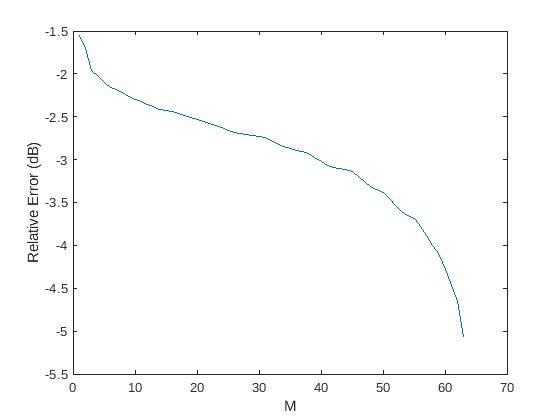
\includegraphics[width=3.2in]{2-c1.jpg}
    \caption{Relative Error vs M}
\end{figure}

\begin{figure}[!ht]
    \subfloat[]{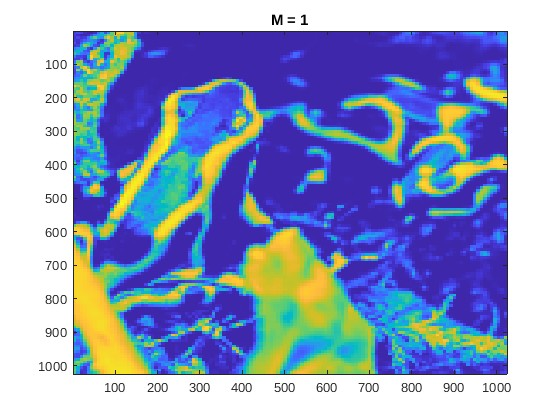
\includegraphics[width=3.2in]{2-c2.jpg}}
    \subfloat[]{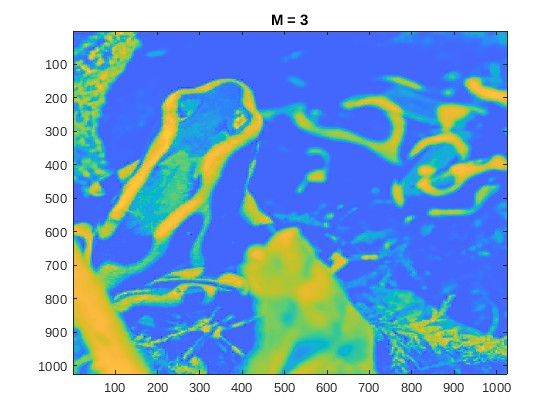
\includegraphics[width=3.2in]{2-c3.jpg}} \\
    \subfloat[]{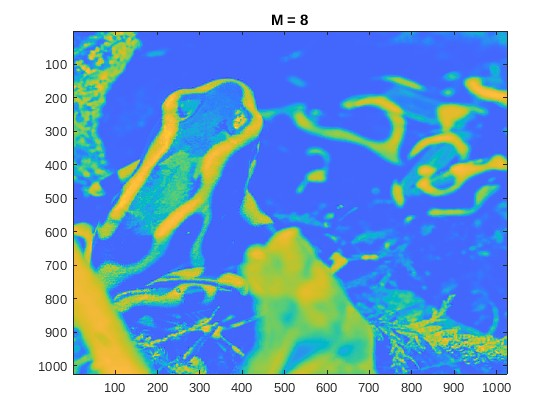
\includegraphics[width=3.2in]{2-c4.jpg}}
    \subfloat[]{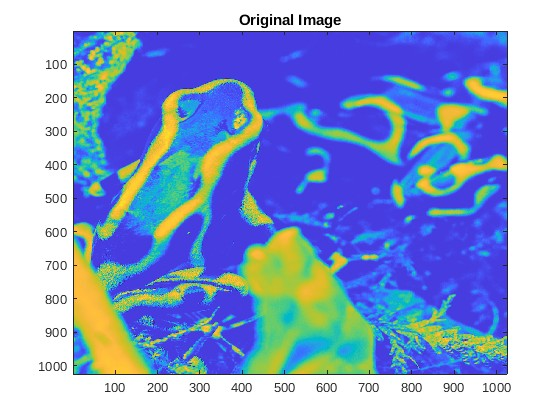
\includegraphics[width=3.2in]{2-c5.jpg}}
    \caption{Image Approximations w/ Various Values of M}
    \centering
\end{figure}

\newpage

\item[d.] Approximation Error w/ Quantized Coefficients

\begin{framed}
$\log_{10}(\frac{\|x-\tilde{x}\|_2^2}{\|x\|_2^2}) = -2.725574$ dB

Number of Non-Zero Coefficients: 96,372 (out of 1,048,576 total)

$\| \tilde{\alpha}-\alpha \| = 4,283.456$

$\| \tilde{x}-x \| = 4,283.456$

$\therefore \| \tilde{\alpha}-\alpha \| = \| \tilde{x}-x \|$
\end{framed}

\newpage

\begin{figure}[!ht]
    \subfloat[]{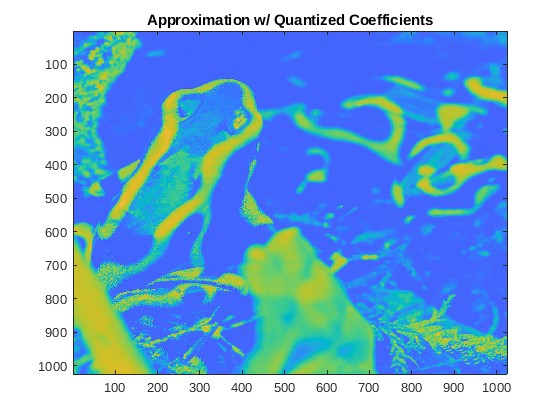
\includegraphics[width=3.2in]{2-c6.jpg}}
    \subfloat[]{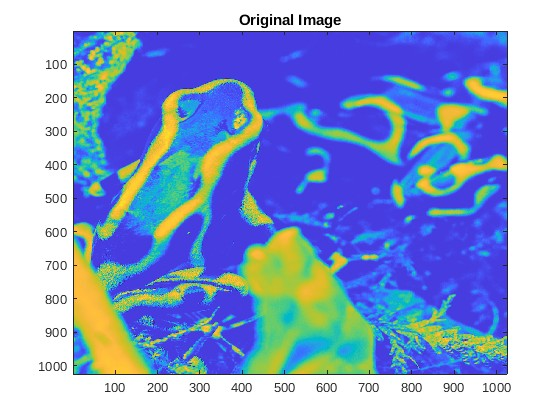
\includegraphics[width=3.2in]{2-c5.jpg}}
    \caption{Image Approximations w/ Quantization Matrix}
    \centering
\end{figure}

DCT With Quantized Coefficients
\begin{lstlisting}[language=matlab]
function [IM_C, COEFF] = block_dct2_approx_quant(IM)
    N = 8;    
    coeffs = block_dct2(IM, N);
    dim = size(coeffs);
    [z, pairs, map] = jpgzzind(dim(1), dim(2));
    load("jpeg_Qtable.mat");
    COEFF = zeros(dim(1), dim(2));
    rows = dim(1) / N;
    cols = dim(2) / N;

    for i = 1:rows
        for j = 1:cols
            COEFF((i-1)*N+1:i*N, (j-1)*N+1:j*N) = Q.*round(coeffs((i-1)*N+1:i*N, (j-1)*N+1:j*N)./Q);
        end
    end

    IM_C = block_idct2(COEFF, N);
end
\end{lstlisting}

\newpage

Calculations
\begin{lstlisting}[language=matlab]
img = double(imread("frog.tiff")) - 128;

[img_approx, coeffs] = block_dct2_approx_quant(img);

error = log10(norm(img-img_approx, 'fro')^2/norm(img, 'fro')^2);
n = nnz(coeffs);
error1 = norm(coeffs-block_dct2(img, 8), 'fro');
error2 = norm(img_approx-img, 'fro');
fprintf("Number of Non-Zero Coefficients = %d\n", n);
fprintf("|a_approx - a| = %d\n", error1);
fprintf("|x_approx - x| = %d\n", error2);
fprintf("Relative Error (dB) = %d\n", error);


figure(1);
imagesc(img_approx);
title("Approximation w/ Quantized Coefficients");
figure(2);
imagesc(img); 
title("Original Image");
hold off;
\end{lstlisting}

\end{enumerate}

\item[Problem 5.3] DCT Implementation

\begin{lstlisting}[language=matlab]
x = randn(100000,1);
d1 = mydct(x);
d2 = dct(x);
norm(d1-d2)

y = randn(100000,1);
w1 = myidct(y);
w2 = idct(y);
norm(w1-w2)
\end{lstlisting}

\begin{framed}
$\|d1-d2\| = 1.3122e-13$

$\|w1-w2\| = 1.3408e-13$
\end{framed}

\newpage

DCT Implementation w/ FFT
\begin{lstlisting}[language=matlab]
function Y = mydct(X)
up_sym_ex = upsample([X; flip(X)], 2, 1);
coeffs = real(fft(up_sym_ex));
Y = coeffs(1:length(X)).*sqrt(1/(2*length(X)));
Y(1) = Y(1)*sqrt(1/2);
end

% PSEUDO-CODE
% Given signal X with N elements
% Create symmetric extension of X
%   - If X = [a b], then the symmetric extension is [a b b a]
% Upsample symmetric extension by two with zeros such that
% every even index = 0
%   - If X_ex = [a b b a], then the upsampled version is [0 a 0 b 0 b 0 a]
% Take FFT of upsampled symmetric extension
% Keep only first N elements of the FFT
% Multiply coeffs where k != 0 by sqrt(2/(N*4))
% Multiply coeff where k = 0 by sqrt(1/(N*4))
\end{lstlisting}

IDCT Implementation w/ IFFT
\begin{lstlisting}[language=matlab]
function X = myidct(Y)
Y_s = Y.*sqrt(length(Y)*2);
Y_s(1) = Y_s(1)*sqrt(2);
odd_ext = [Y_s; 0; -flip(Y_s)];
coeffs = [odd_ext(1:end-1); -odd_ext(1:end-1)];
X = ifft(coeffs);
X = downsample(X(1:2*length(Y)),2,1);
end

% PSEUDO-CODE
% Given DCT coefficients Y with N elements
% Scale coeffs where k != 0 by sqrt((4*N)/2))
% Scale coeff where k = 0 by sqrt(4*N)
% Flip and tile coefficients so they match fft
%   - If Y = [a b c], then the fft coeffs [a b c 0 -c -b -a -b -c 0 c b]
% Take the inverse FFT of the tiled and flipped coeffs
% Take the first N*2 elements of X and downsample by 2
%   - ifft(coeffs) = [0 a 0 b 0 c 0 d], so X = [a b c d]
\end{lstlisting}

\end{enumerate}


\end{document}
